\documentclass[12pt,a4paper]{article}
\usepackage{amsmath,amscd,amsbsy,amssymb,latexsym,url,bm,amsthm}
\usepackage{epsfig,graphicx,subfigure}
\usepackage{enumitem,balance}
\usepackage{wrapfig}
\usepackage{mathrsfs,euscript}
\usepackage[usenames]{xcolor}
\usepackage{hyperref}
\usepackage[vlined,ruled,linesnumbered]{algorithm2e}
\usepackage{array}
\hypersetup{colorlinks=true,linkcolor=black}

\newtheorem{theorem}{Theorem}
\newtheorem{lemma}[theorem]{Lemma}
\newtheorem{proposition}[theorem]{Proposition}
\newtheorem{corollary}[theorem]{Corollary}
\newtheorem{exercise}{Exercise}
\newtheorem*{solution}{Solution}
\newtheorem{definition}{Definition}
\theoremstyle{definition}

\renewcommand{\thefootnote}{\fnsymbol{footnote}}

\newcommand{\postscript}[2]
 {\setlength{\epsfxsize}{#2\hsize}
  \centerline{\epsfbox{#1}}}

\renewcommand{\baselinestretch}{1.0}

\setlength{\oddsidemargin}{-0.365in}
\setlength{\evensidemargin}{-0.365in}
\setlength{\topmargin}{-0.3in}
\setlength{\headheight}{0in}
\setlength{\headsep}{0in}
\setlength{\textheight}{10.1in}
\setlength{\textwidth}{7in}
\makeatletter \renewenvironment{proof}[1][Proof] {\par\pushQED{\qed}\normalfont\topsep6\p@\@plus6\p@\relax\trivlist\item[\hskip\labelsep\bfseries#1\@addpunct{.}]\ignorespaces}{\popQED\endtrivlist\@endpefalse} \makeatother
\makeatletter
\renewenvironment{solution}[1][Solution] {\par\pushQED{\qed}\normalfont\topsep6\p@\@plus6\p@\relax\trivlist\item[\hskip\labelsep\bfseries#1\@addpunct{.}]\ignorespaces}{\popQED\endtrivlist\@endpefalse} \makeatother

\begin{document}
\noindent

%========================================================================
\noindent\framebox[\linewidth]{\shortstack[c]{
\Large{\textbf{Lab08-Computational Complexity}}\vspace{1mm}\\
CS214-Algorithm and Complexity, Xiaofeng Gao, Spring 2019.}}
\begin{center}
\footnotesize{\color{red}$*$ If there is any problem, please contact TA Jiahao Fan or TA Mingran Peng.}

% Please write down your name, student id and email.
\footnotesize{\color{blue}$*$ Name: KylinChen  \quad Student ID: 517030910155 \quad Email: k1017856853@icloud.com}
\end{center}

\begin{enumerate}
    \item
    Design a one-tape TM $M$ that computes the function $f(x, y) = x - y$, where $x$ and $y$ are positive integers ($x > y$). The alphabet is $\{1, 0, \Box, \triangleright, \triangleleft\}$, and the inputs are $x$ 1's, $\Box$ and $y$ 1's. Below is the initial configuration for input $x=7$ and $y=3$. The result $z=f(x, y)$ should also be represented in the form of $z$ 1's on the tape with the pattern of $\triangleright 111 \cdots 111 \triangleleft$.

    \begin{center}
    \begin{tabular}{ll|c|c|c|c|c|c|c|c|c|c|c|c|c|c}
    	\cline{2-16}
    	Init:& & $\triangleright$ &  1  & 1 & 1 & 1 & 1 & 1 & 1 & $\Box$ & 1 & 1 & 1 & $ \triangleleft$ & \\
    	\cline{2-16}
    	\multicolumn{2}{c}{} & \multicolumn{1}{c}{$\uparrow$} & \multicolumn{11}{c}{}\\
    	\multicolumn{2}{c}{} & \multicolumn{1}{c}{$q_S$} & \multicolumn{11}{c}{}\\
    \end{tabular}
    \end{center}

    \begin{enumerate}
        \item
        Please describe your design and then write the specifications of $M$ in the form like $\langle q_S, \triangleright \rangle \rightarrow \langle q_1, \triangleright,  R\rangle$. Explain the transition functions in detail.

        \item
        Please draw the state transition diagram using Microsoft Visio.

        \item
        Show briefly and clearly the whole process from initial to final configurations for input $x = 7$ and $y = 3$.
    \end{enumerate}

    \begin{solution}\item
    \renewcommand{\qedsymbol}{}
    \begin{itemize}
    \item [(a)] 
    \begin{itemize}
    \item For one-tape TM M, the reading head $q$ may write a symbol, move left, move right. The we give our state-transfer prototype as:
    $$\langle q_i , s_w \rangle \rightarrow \langle q_j , s_k , L/R/S\rangle$$
    which means reading head state transfer: $q_{i} \rightarrow q_{j}$, tape value replace $s_w$ with $s_k$, reading head movement is $L$(Left) / $R$(Right) / $S$(Stand Still).
    \item Define state $q_{i}$:\par 
    $q_{S}$: start/right move state; $q_{E}$: end/return front state; $q_{H}$: Halt state(refering to Powpoint, we set $q_{H}$ at the first letter rather than $\triangleright$); $q_{1}$: delete $y$ 1's state; $q_{2}$: left move state; $q_{3}$: delete $x$ 1's state;
    \item Given a Turing machine M state-transfer table:
    $$\langle q_s , \triangleright \rangle \rightarrow \langle q_s , \triangleright , R\rangle,\ \ \ \ \  \ \langle q_s , 1 \rangle \rightarrow \langle q_s , 1 , R\rangle$$
    $$\langle q_s , \Box \rangle \rightarrow \langle q_s , \Box , R\rangle,\ \ \ \ \  \ \langle q_s , \triangleleft \rangle \rightarrow \langle q_1 , \Box , L\rangle$$
    $$\langle q_1 , 1 \rangle \rightarrow \langle q_2 , \triangleleft , S\rangle,\ \ \ \ \  \ \langle q_1 , \Box \rangle \rightarrow \langle q_E , \triangleleft , S\rangle$$
    $$\langle q_2 , \triangleleft \rangle \rightarrow \langle q_2 , \triangleleft , L\rangle,\ \ \ \ \  \ \langle q_2 , 1 \rangle \rightarrow \langle q_2 , 1 , L\rangle$$
    $$\langle q_2 , \Box \rangle \rightarrow \langle q_2 , \Box , L\rangle,\ \ \ \ \  \ \langle q_2 , \triangleright \rangle \rightarrow \langle q_3 , \Box , R\rangle$$
    $$\langle q_3 , 1 \rangle \rightarrow \langle q_s , \triangleright , S\rangle,\ \ \ \ \  \ \langle q_E , \triangleleft \rangle \rightarrow \langle q_E , \triangleleft , L\rangle$$
    $$\langle q_E , 1 \rangle \rightarrow \langle q_E , 1 , L\rangle,\ \ \ \ \  \ \langle q_E , \triangleright \rangle \rightarrow \langle q_H , \triangleright , R\rangle$$
    \end{itemize}
    \item [(b)] We can use $Microsoft\ Visio\ 2013$ to draw the state transition diagram below, the $visio$ file $TM.vsdx$ is attach in .zip file folder. Its export TM.pdf can be as Figure.~\ref{Graph0}
    \begin{figure}[htbp]
        \centering
        \includegraphics[width=0.8\textwidth]{pictures/TM.pdf}
        \caption{\textbf{State Transition Diagram by Microsoft Visio 2013}}\label{Graph0}
    \end{figure}
    \item [(c)] For the given example, whose initial configuration is set for input x = 7 and y = 3, and put reading head $q_{S}$ at front $\triangleright$, we can give the TM M compute process as Figure.\ref{Graph1}\par (In the computation process, we leave out some loop to list the key steps instead)
    \begin{figure}[htbp]
        \centering
        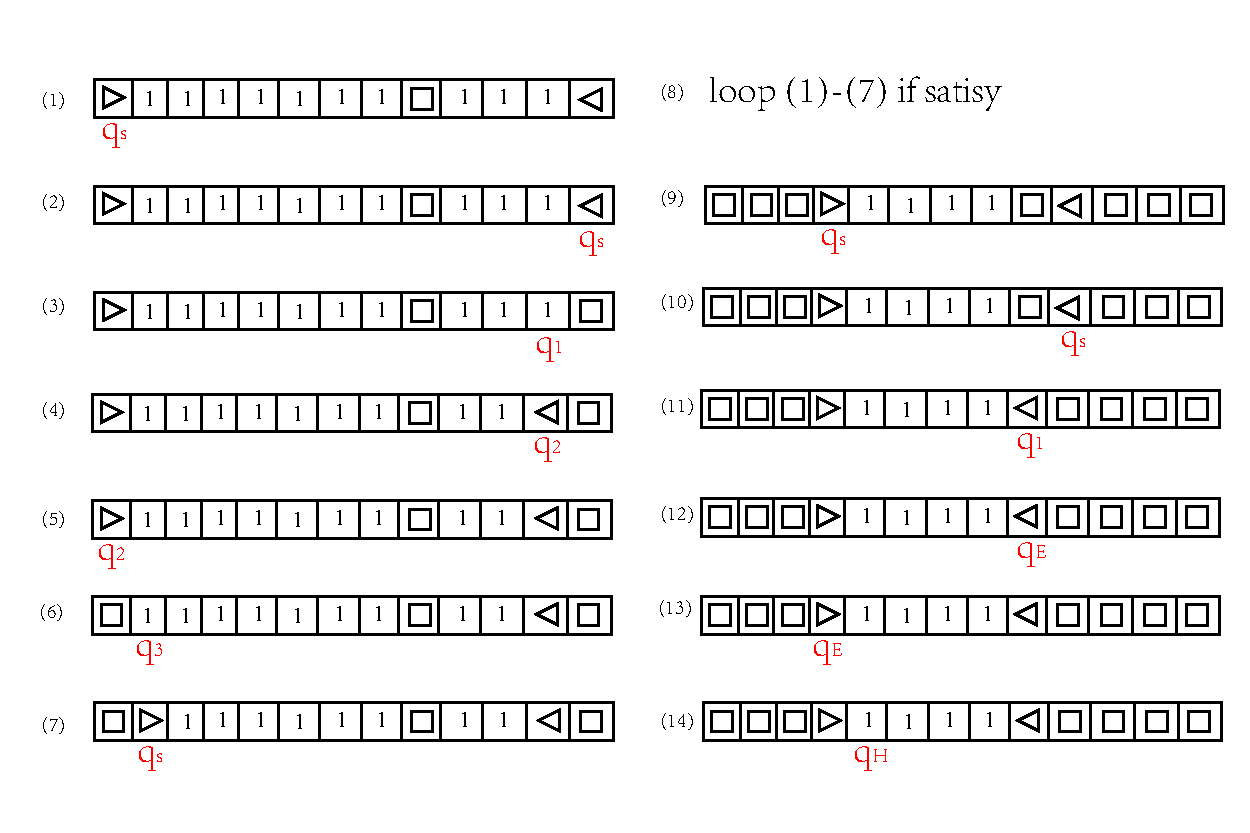
\includegraphics[width=0.8\textwidth]{pictures/pic_1.pdf}
        \caption{\textbf{TM Computation Process}}\label{Graph1}
    \end{figure}
    \end{itemize}
    \end{solution}

    \item
    What is the ``certificate'' and ``certifier'' for the following problems?
    \begin{enumerate}
        \item
        \emph{PARTITION}: Given a finite set $A$ and a size $s(a) \in \mathbb{Z}$ for each $a \in A$, is there a subset $A' \subseteq A$ such that $\sum_{a \in A'}s(a) = \sum_{a \in A-A'}s(a)$ ?

        \item
        \emph{CLIQUE}: Given a graph $G = (V, E)$ and a positive integer $K \leq |V|$, is there a subset $V' \subseteq V$ with $|V'| \geq K$ such that every two vertices in $V'$ are joined by an edge in $E$ ?

        \item
        \emph{ZERO-ONE INTEGER PROGRAMMING}: Given an integer $m \times n$ matrix $A$ and an integer $m$-vector $b$, is there an integer $n$-vector $x$ with elements in the set $\{0, 1\}$ such that $Ax \leq b$ ?
    \end{enumerate}

    \begin{solution}\item
    \renewcommand{\qedsymbol}{}
    \begin{itemize}
    \item [(a)] \textbf{certificate:} A certificate is a subset $A' \in A$, which satisfys the problem requirements, note that such a certificate exists iff problem requirements can be satified.\par
    \textbf{certifier:} \par 
        \begin{minipage}[t]{0.8\textwidth}
        \begin{algorithm}[H]
            \KwIn{$set$ A; $set$ A';}
            \KwOut{$bool$ res;}
            %\BlankLine
            \caption{$certifier\ 1$}
            \label{ALG1}
            $count \leftarrow 0$\;
            \For{item $a \in A$}{
                \If{$a \in A'$}{$count \leftarrow count+s(a) $\;}
                \Else{$count \leftarrow count-s(a) $\;}
            }
            return $(count==0)$\;

        \end{algorithm}
        \end{minipage}
        \hfill
    \item [(b)] \textbf{certificate:} A certificate is a k-node set $N' \in N$, which satisfys the problem requirements, note that such a certificate exists iff all node pair in $N'$ have connected by at least one edge $e$ ($e \in E$).\par
    \textbf{certifier:} \par 
        \begin{minipage}[t]{0.8\textwidth}
        \begin{algorithm}[H]
            \KwIn{$set$ A; $set$ A';}
            \KwOut{$bool$ res;}
            %\BlankLine
            \caption{$certifier\ 2$}
            \label{ALG2}
            \For{node $i \in N'$}{
                \For{node $j \in N'/\{j\}$}{
                    \If{$Connect(i,j)==False$}{return $False$\;}
                } 
            }
            return $True$\;

        \end{algorithm}
        \end{minipage}
        \hfill
    \item [(c)] \textbf{certificate:} A certificate is a n-vector $x$, which satisfys the problem requirements, note that such a certificate exists iff $Ax \leq b$.\par
    \textbf{certifier:} \par 
        \begin{minipage}[t]{0.8\textwidth}
        \begin{algorithm}[H]
            \KwIn{$set$ A; $set$ A';}
            \KwOut{$bool$ res;}
            %\BlankLine
            \caption{$certifier\ 3$}
            \label{ALG3}
            \For{$i\leftarrow 1$ \textbf{to} $m$}{
                $A[i] \leftarrow A's\ \text{i-th}\ row $\;
                \If{$A[i]\cdot x > b[i]$}{return $False$\;}
            }
            return $True$\;

        \end{algorithm}
        \end{minipage}
        \hfill
    \end{itemize}
    \end{solution}

    \item
    \emph{SUBSET SUM}: Given a finite set $A$, a size $s(a) \in \mathbb{Z}$ for each $a \in A$ and an integer $B$, is there a subset $A' \subseteq A$ such that $\sum_{a \in A'}s(a) = B$?

    \emph{KNAPSACK}: Given a finite set $A$, a size $s(a) \in \mathbb{Z}$ and a value $v(a) \in \mathbb{Z}$ for each $a \in A$ and integers $B$ and $K$, is there a subset $A' \subseteq A$ such that $\sum_{a \in A'}s(a) \leq B$ and $\sum_{a \in A'}v(a) \geq K$?

    \begin{enumerate}
    \item
    Prove \emph{PARTITION} $\leq_p$ \emph{SUBSET SUM}.

    \item
    Prove \emph{SUBSET SUM} $\leq_p$ \emph{KNAPSACK}.

    \end{enumerate}

    \begin{proof}\item
    \renewcommand{\qedsymbol}{}
    \begin{itemize}
    \item [(a)]
    \begin{itemize}
        \item Instance of Set Partition: Given Set $A$.
        \par Instance of Subset Sum: Same Set $A$, aimed sum $B$.

        \item To Prove:\par
        $\Rightarrow $ There exist a aimed sum $B'$, which makes Set Partition problem become a Subset Sum problem.\par
        $\Leftarrow $ Subset Sum problem can be specified into a Set Partition problem.

        \item Prove:\par
        For Given Set $A$, we can compute $\Theta = \sum_{a=1}^{|A|}s(a)$, then make $B'=\frac{1}{2}\Theta$. $A'$ have the same value with $A-A'$ $\Rightarrow$ $A'$ have the aimed value $B'$.
    \end{itemize}
    \item [(b)]
    \begin{itemize}
        \item Instance of Subset Sum: Same Set $A$, aimed sum $B_{1}$.
        \par Instance of Knapsack: Same Set $A$, size upper bounder $B_{2} $, value lower bounder $K $.

        \item To Prove:\par
        $\Rightarrow $ There exist $B_{2}$, $K$ and function $v(a)$, which makes Subset Sum problem become a Knapsack problem.\par
        $\Leftarrow $ Knapsack problem can be specified into a Subset Sum problem.

        \item Prove:\par
        For Given Set $A$, we can set $B_{2}=K=B_{1}$, function $v=s$ $\Leftarrow $ $\sum_{a \in A'}s(a) \leq B_{2}$ and $\sum_{a \in A'}s(a) \geq B_{2} $ $\Rightarrow $ $\sum_{a \in A'}s(a) = B_{2} $, this is subset sum problem.
    \end{itemize}
    \end{itemize}
    \end{proof}

    \item
    \emph{3-SAT}: Given a set $U$ of variables, a collection $C$ of clauses over $U$ such that each clause $c \in  C$ has $|c| = 3$, is there a satisfying truth assignment for $C$?

    Prove \emph{3-SAT} $\leq_p$ \emph{CLIQUE}.
    \begin{proof}\item
    \renewcommand{\qedsymbol}{}
    \begin{itemize}
    \item \textbf{Configuration.} Since we want to prove a reduction between logic problem($3-SAT$) and graph problem($k$-CLIQUE), we must establish a graph model $G$ between them, which satisfys: it have nodes for all (clause, literal) pairs and edges between all non-contradictory nodes in different clauses.
    \item \textbf{Claim.} $3-SAT$ satisfiable iff $G$ has a $k$-CLIQUE.
    \item \textbf{Example.} We give a synergy paradigm below:
    $$w = (x_1 \vee x_2 \vee x_3) \wedge (\neg x_1 \vee x_2 \vee \neg x_3) \wedge (\neg x_1 \vee \neg x_2 \vee \neg x_3)$$
    For general, $k$ represent number of clauses, in this case, $k=3$, We label them with $c_1, c_2, c_3 $ in this example.\par
    We can draw the graph model in Figure.\ref{Graph2}
    \begin{figure}[htbp]
        \centering
        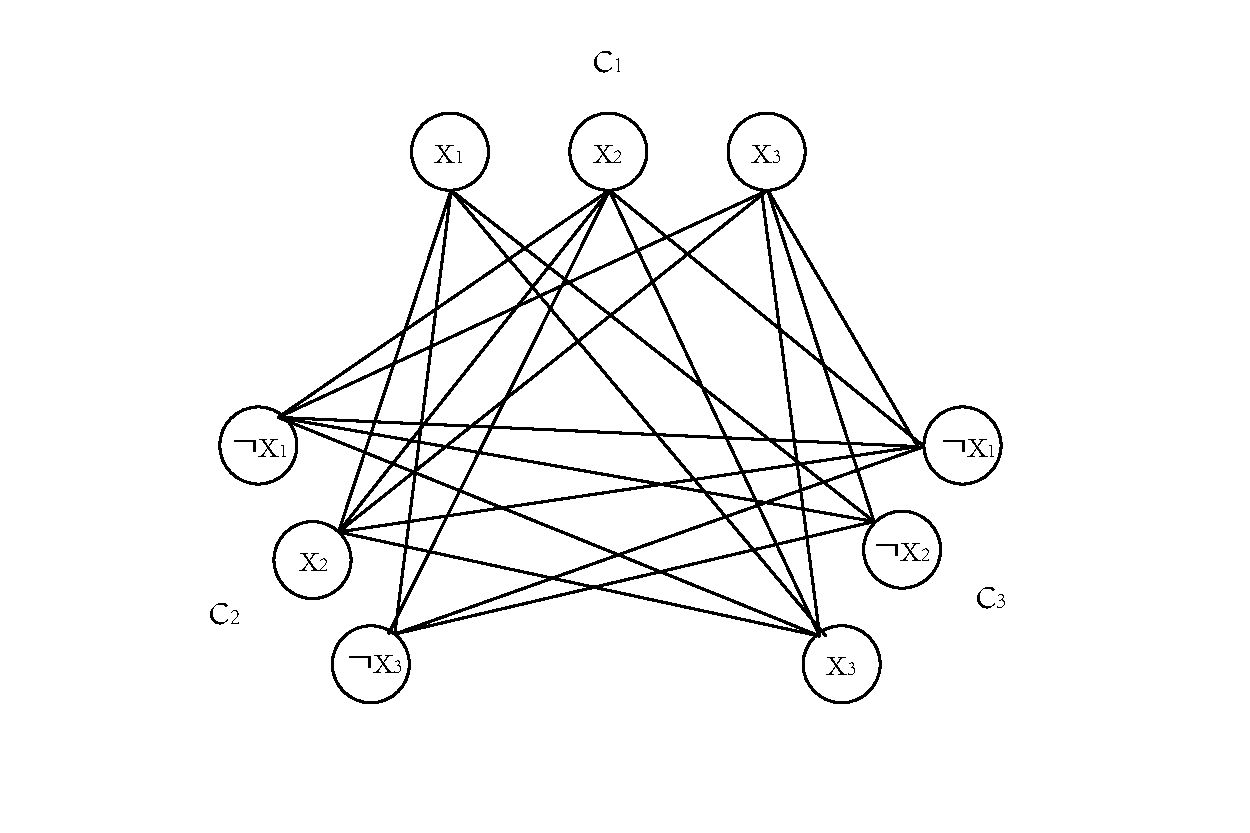
\includegraphics[width=0.5\textwidth]{pictures/pic_2.pdf}
        \caption{\textbf{Graph Model G for The Example}}\label{Graph2}
    \end{figure}

    We can pick a 3-KLIQUE($k=3$) to see its correctness. (In Figure.\ref{Graph3}, red-line CLIQUE).\par
    Once this CLIQUE exists, we can set all nodes in this CLIQUE $True$, which means:
    $$x_1=False, x_2=False, x_3=True$$ which satisfys 3-SAT.

    \begin{figure}[htbp]
        \centering
        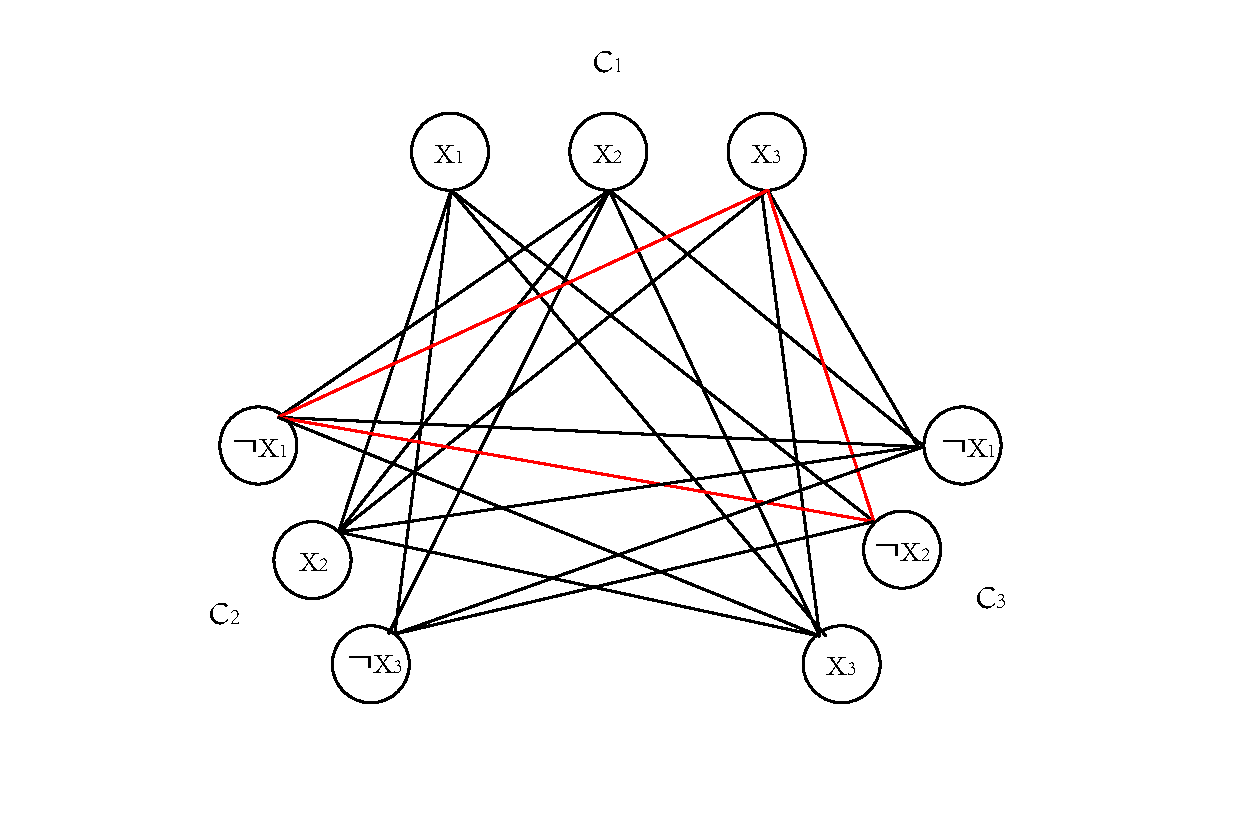
\includegraphics[width=0.5\textwidth]{pictures/pic_3.pdf}
        \caption{\textbf{A Certificate Clique}}\label{Graph3}
    \end{figure}


    \item \textbf{To Prove.} $3-SAT$ satisfiable iff $G$ has a $k$-CLIQUE.
    \item \textbf{Prove.} \par
    \textbf{$\Rightarrow: $} Assume the formula is satisfiable which means satisfying assignment gives one literal in each clause, all with non-contradictory assignments. Therefore, it yields a k-clique, which makes one $True$ literal in every clause satisfied.
    \par\textbf{$\Leftarrow: $} Assume there is a k-clique in Graph model G, which yields one node per clause, none contradictory. Once at least one $k$-CLIQUE exist, it yeilds more than one consistent assignments satisfying all clauses of synergy paradigm w and make 3-SAT established.
    \end{itemize}
    \end{proof}

\item Algorithm class is a democratic class. Denote class as a finite set $S$ containing every students. Now students decided to raise a student union $S' \subseteq S$ with $|S'|\leq K$ .\par
As for the members of the union, there are many different opinions. An opinion is a set $S_o\subseteq S$. Note that number of opinions has nothing to do with number of students.\par
The question is whether there exists such student union $S' \subseteq S$ with $|S'|\leq K$, that $S'$ contains at least one element from each opinion. We call this problem \emph{ELECTION} problem, prove that it is NP-complete.

\begin{proof}\item
\renewcommand{\qedsymbol}{}
\begin{itemize}
\item \textbf{Configuration}:
\begin{itemize}
\item $S$ contains $n$ elements(students).
\item There are $m$ kinds of opinion subsets $S_{0}$, marked with $S_{0(1)} $, $S_{0(2)} $, $S_{0(3)} $, $\cdots S_{0(m)} $.
\end{itemize}
\item \textbf{ELECTION $\in$ NP}:\par To Prove ELECTION $\in$ NP, we need to claim there is a poly-time certifier $C(S, t)$. For any subset $S'\in S$, $C(S', t)=True$ iff $S'$ contains at least one elements of every opinion subset $S_{0}$. Vise verse. \par
$\Rightarrow $ Once we have a subsets $S' \in S$, we can use brute-force to check whether $S'$ contains at least one elements in $S_{0(t)} $, it takes $O(n^2)$ for each $S_{0}$ check, it means for certificier $C(S, t)$, $t = O(mn^2)$, which confirm to poly-time constarin. Therefore, ELECTION $\in$ NP problem.
\item \textbf{Set-Covering $\leq_p$ ELECTION}: \par
Set-Covering Problem belongs to Karp's 21 NP-complete problems, it means:
$$Set-Covering \in NPC$$
According to proven Claim: \par
$$X \in NPC,\ \ Y \in NP,\ \ X \leq_p Y \Rightarrow Y \in NPC.$$
$ELECTION \in NP$ is given above. So we need to prove Set-Covering $\leq_p$ ELECTION:\par
$\Rightarrow $: For every element $s_{w}$ in S, it may be contained by several opinion subset: $$s_{w} \in S_{0(t)}, \forall w\in \{1, \cdots n\}\ (\ for\ some\ t\in \{1, \cdots m\} , w  \in  \{1, \cdots n\}\ )  $$ It can be marked:
$$C_{w} = \{S_{0(t)} \cdots \}\ \ (for\ some\ t \ \in \ \{1, \cdots m\} )$$
$C_{w}$ means the set of set which contains $s_{w}$, and $C_{w}$ can be $\emptyset$ iff $s_{w}$ isn't contained in any opinion subset $S_{0(t)} ( \forall t  \in  \{1, \cdots m\} )$.\par

Then, we can get the universe set: $$U=\{S_{0(1)} ,\ S_{0(2)} ,\ S_{0(3)} ,\ \cdots\ S_{0(m)}\} $$
And the collection of sets
$$C_u=\{C_{1},\ C_{2},\ C_{3},\ C_{4},\cdots\ C_{n} \}$$
Then, ELECTION problem is converted into Set-Covering problem, aimed to cover the universe set $U$ with setset union of $C_{u}$. And, origin ELECTION problem exist satisfied answer iff Set-Covering exist a collection of $\leq K$ of these sets whose union is equal to $C_{u}$.\par
$\Leftarrow $(correctness): Once these sets' union is equal to $C_{u}$, it means all the opinion subset have at least one elements in the colection union. Moreover, the colection $\leq K$ means we selection no more than K elements, which confirms to origin ELECTION problem.
\item \textbf{Example}: \par
We give a example like Figure.\ref{Graph4}. There are four opinions and six students, and An edge between opinion and student means this opinion construct an union which contains this student, for instance, in this case(Figure.\ref{Graph4}), opinion1 construct an union containing student1, student2 and student3.\par
Then, we can number these opinion with 1 to 4, which are combined to universe set $U$.  \color{red}(In my proof above, opinion1(include other opinions) is a set like \{1,2,3\}, and $C_{1}$ contains this set as an element, but we simplify it in our example.)\color{black}\par
Moreover, we can construct a set $C_{i}$ for each student $i$, once this student belongs to this opinion sebset, for example, $C_{1}=\{1,2,3\}$ since these three opinion want to invite student1 to their own union. Finally, we can convert our problem to: Can we find no more than $k$ subsets in $G_{u}$, which covers $U$. THis is obviously a NP-complete problem, so is the origin problem.
\begin{figure}[htbp]
        \centering
        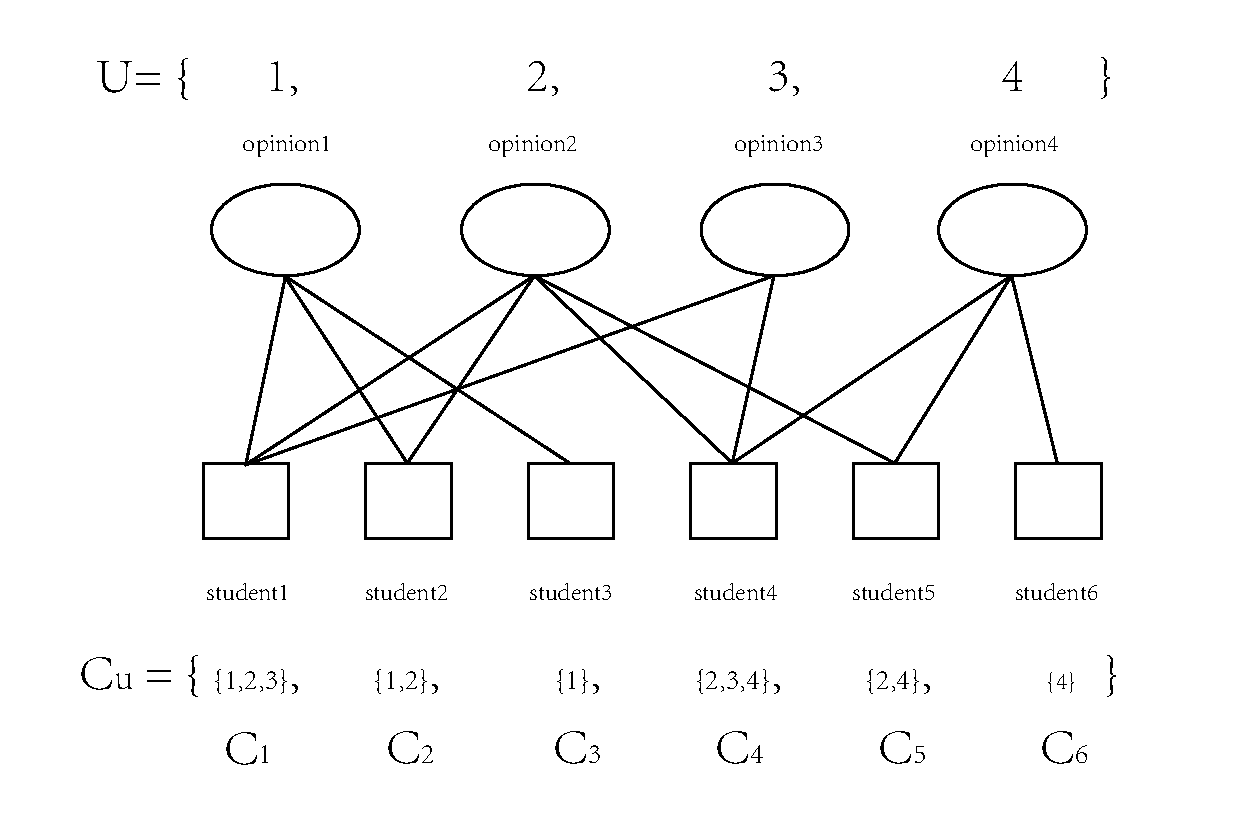
\includegraphics[width=0.7\textwidth]{pictures/pic_4.pdf}
        \caption{\textbf{How to build U and $C_{u}$}}\label{Graph4}
\end{figure}
\end{itemize}
\end{proof}

\end{enumerate}

\vspace{20pt}



%========================================================================
\end{document}
